\section{Описание модели}
	Структурная схема модели представленна на рисунке \ref{pic:scheme}.
	
	\begin{figure}[h]
		\begin{center}
			{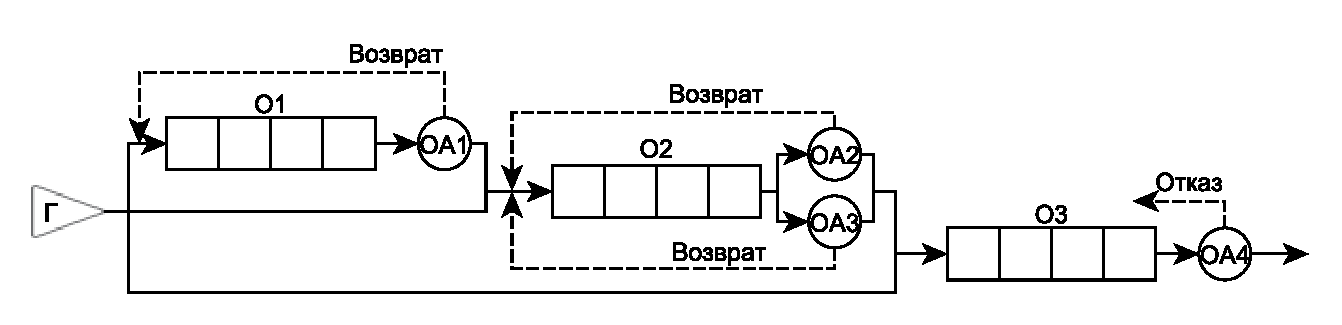
\includegraphics[scale=0.7]{СМО.pdf}
				\caption{Структурная схема модели}
				\label{pic:scheme}}
		\end{center}
	\end{figure}
	\pagebreak
	Согласно условию время обработки студента магистрами и преподавателем подчиняется закону равномерного распределения. Автоматы обслуживания в модели классифицируются следующим образом:
	\begin{itemize}
		\item ОА1, ОА2, ОА3 - АО, симулирующие работу магистров.
		\item ОА4 симулирует работу преподавателя.
	\end{itemize}

	Эндогенными переменными системами являются время обработки студентов для магистров и преподавателя. 
	
	Экзогенными являются число студентов, которые получили и не получили зачёт, пиковая длина каждой из очередей.


\section{Работа программы}	
	Результаты моделирования приведены на рисунке \ref{pic:res}.
	
	\begin{figure}[h]
		\begin{center}
			{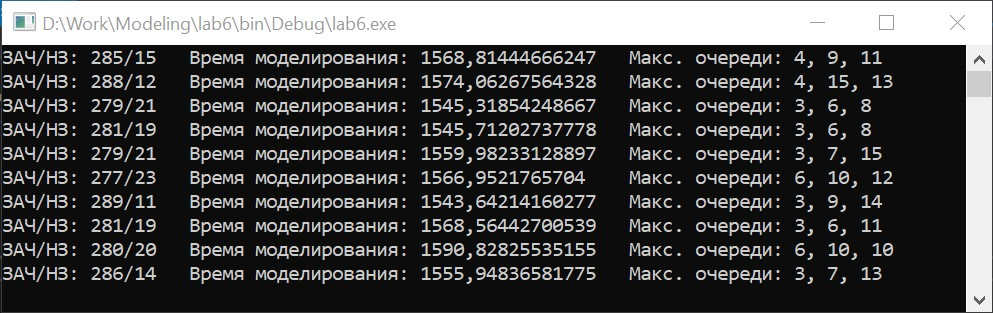
\includegraphics[scale=0.85]{result.jpg}
				\caption{Пример работы программы}
				\label{pic:res}}
		\end{center}
	\end{figure}
	